\documentclass[
  bibliography=totoc,     % Literatur im Inhaltsverzeichnis
  captions=tableheading,  % Tabellenüberschriften
  titlepage=firstiscover, % Titelseite ist Deckblatt
]{scrartcl}

% Paket float verbessern
\usepackage{scrhack}

% Warnung, falls nochmal kompiliert werden muss
\usepackage[aux]{rerunfilecheck}

% unverzichtbare Mathe-Befehle
\usepackage{amsmath}
% viele Mathe-Symbole
\usepackage{amssymb}
% Erweiterungen für amsmath
\usepackage{mathtools}

% Fonteinstellungen
\usepackage{fontspec}
% Latin Modern Fonts werden automatisch geladen
% Alternativ zum Beispiel:
%\setromanfont{Libertinus Serif}
%\setsansfont{Libertinus Sans}
%\setmonofont{Libertinus Mono}

% Wenn man andere Schriftarten gesetzt hat,
% sollte man das Seiten-Layout neu berechnen lassen
\recalctypearea{}

% deutsche Spracheinstellungen
\usepackage{polyglossia}
\setmainlanguage{german}


\usepackage[
  math-style=ISO,    % ┐
  bold-style=ISO,    % │
  sans-style=italic, % │ ISO-Standard folgen
  nabla=upright,     % │
  partial=upright,   % ┘
  warnings-off={           % ┐
    mathtools-colon,       % │ unnötige Warnungen ausschalten
    mathtools-overbracket, % │
  },                       % ┘
]{unicode-math}

% traditionelle Fonts für Mathematik
\setmathfont{Latin Modern Math}
% Alternativ zum Beispiel:
%\setmathfont{Libertinus Math}

\setmathfont{XITS Math}[range={scr, bfscr}]
\setmathfont{XITS Math}[range={cal, bfcal}, StylisticSet=1]

% Zahlen und Einheiten
\usepackage[
  locale=DE,                   % deutsche Einstellungen
  separate-uncertainty=true,   % immer Fehler mit \pm
  per-mode=symbol-or-fraction, % / in inline math, fraction in display math
]{siunitx}

% chemische Formeln
\usepackage[
  version=4,
  math-greek=default, % ┐ mit unicode-math zusammenarbeiten
  text-greek=default, % ┘
]{mhchem}

% richtige Anführungszeichen
\usepackage[autostyle]{csquotes}

% schöne Brüche im Text
\usepackage{xfrac}

% Standardplatzierung für Floats einstellen
\usepackage{float}
\floatplacement{figure}{htbp}
\floatplacement{table}{htbp}

% Floats innerhalb einer Section halten
\usepackage[
  section, % Floats innerhalb der Section halten
  below,   % unterhalb der Section aber auf der selben Seite ist ok
]{placeins}

% Seite drehen für breite Tabellen: landscape Umgebung
\usepackage{pdflscape}

% Captions schöner machen.
\usepackage[
  labelfont=bf,        % Tabelle x: Abbildung y: ist jetzt fett
  font=small,          % Schrift etwas kleiner als Dokument
  width=0.9\textwidth, % maximale Breite einer Caption schmaler
]{caption}
% subfigure, subtable, subref
\usepackage{subcaption}

% Grafiken können eingebunden werden
\usepackage{graphicx}
% größere Variation von Dateinamen möglich
\usepackage{grffile}

% schöne Tabellen
\usepackage{booktabs}

% Verbesserungen am Schriftbild
\usepackage{microtype}

% Literaturverzeichnis
\usepackage[
  backend=biber,
]{biblatex}
% Quellendatenbank
\addbibresource{lit.bib}
\addbibresource{programme.bib}

% Hyperlinks im Dokument
\usepackage[
  unicode,        % Unicode in PDF-Attributen erlauben
  pdfusetitle,    % Titel, Autoren und Datum als PDF-Attribute
  pdfcreator={},  % ┐ PDF-Attribute säubern
  pdfproducer={}, % ┘
]{hyperref}
% erweiterte Bookmarks im PDF
\usepackage{bookmark}

% Trennung von Wörtern mit Strichen
\usepackage[shortcuts]{extdash}

\author{%
  AUTOR A\\%
  \href{mailto:authorA@udo.edu}{authorA@udo.edu}%
  \texorpdfstring{\and}{,}%
  AUTOR B\\%
  \href{mailto:authorB@udo.edu}{authorB@udo.edu}%
}
\publishers{TU Dortmund – Fakultät Physik}


\title{Versuch 103 "Biegung elastischer Stäbe"}

\author{
  Robert Konradi\\%
  \href{mailto:authorA@udo.edu}{robert.konradi@tu-dortmund.de}%
  \texorpdfstring{\and}{,}%
  Lauritz Klünder\\%
  \href{mailto:authorB@udo.edu}{lauritz.kluender@tu-dortmund.de}%
}
\date{Durchführung: 10.11.2017, Abgabe: 17.11.2017}
\publishers{TU Dortmund – Fakultät Physik}
\begin{document}
\maketitle
\setlength{\parindent}{0pt}
%\thispagestyle{empty}
\tableofcontents
\newpage
\section{Einleitung}
Das Trägheitsmoment von verschiedene Körpern soll bestimmt werden und der Satz von Steiner verifiziert werden.
\section{Theorie}
Das Drehmoment $M$, das Trägheitsmoment $I$ als auch die Winkelbeschleunigung \.{\omega} charakterisieren die Rotationsbewegung.
Für eine punktförmige Masse kann das Trägheitsmoment mit $I = m*r^2$ berechnen. Dabei ist m die Masse und r der Abstand zur Drehachse.
Für ein ausgedehnten Körper um eine feste Achse kann das Gesamtträgheitsmoment als:
\begin{equation}
  I=\sum \limits_{i}^{} r_\text{i}^2 \cdot m_\text{i}
\end{equation}
dargestellt werden.
Das Drehmoment $M$ ist von der Lage der Drehachse abhängig.
Für geometrische Objekte, wie ein Kugel, Stab, Zylinder, lässt sich das Trägheitsmoment
leicht bestimmen.
In Abbildung 1 sind verschiedene Objekte mit deren Trägheitsmoment dargestellt.
\begin{figure}[H]
\centering
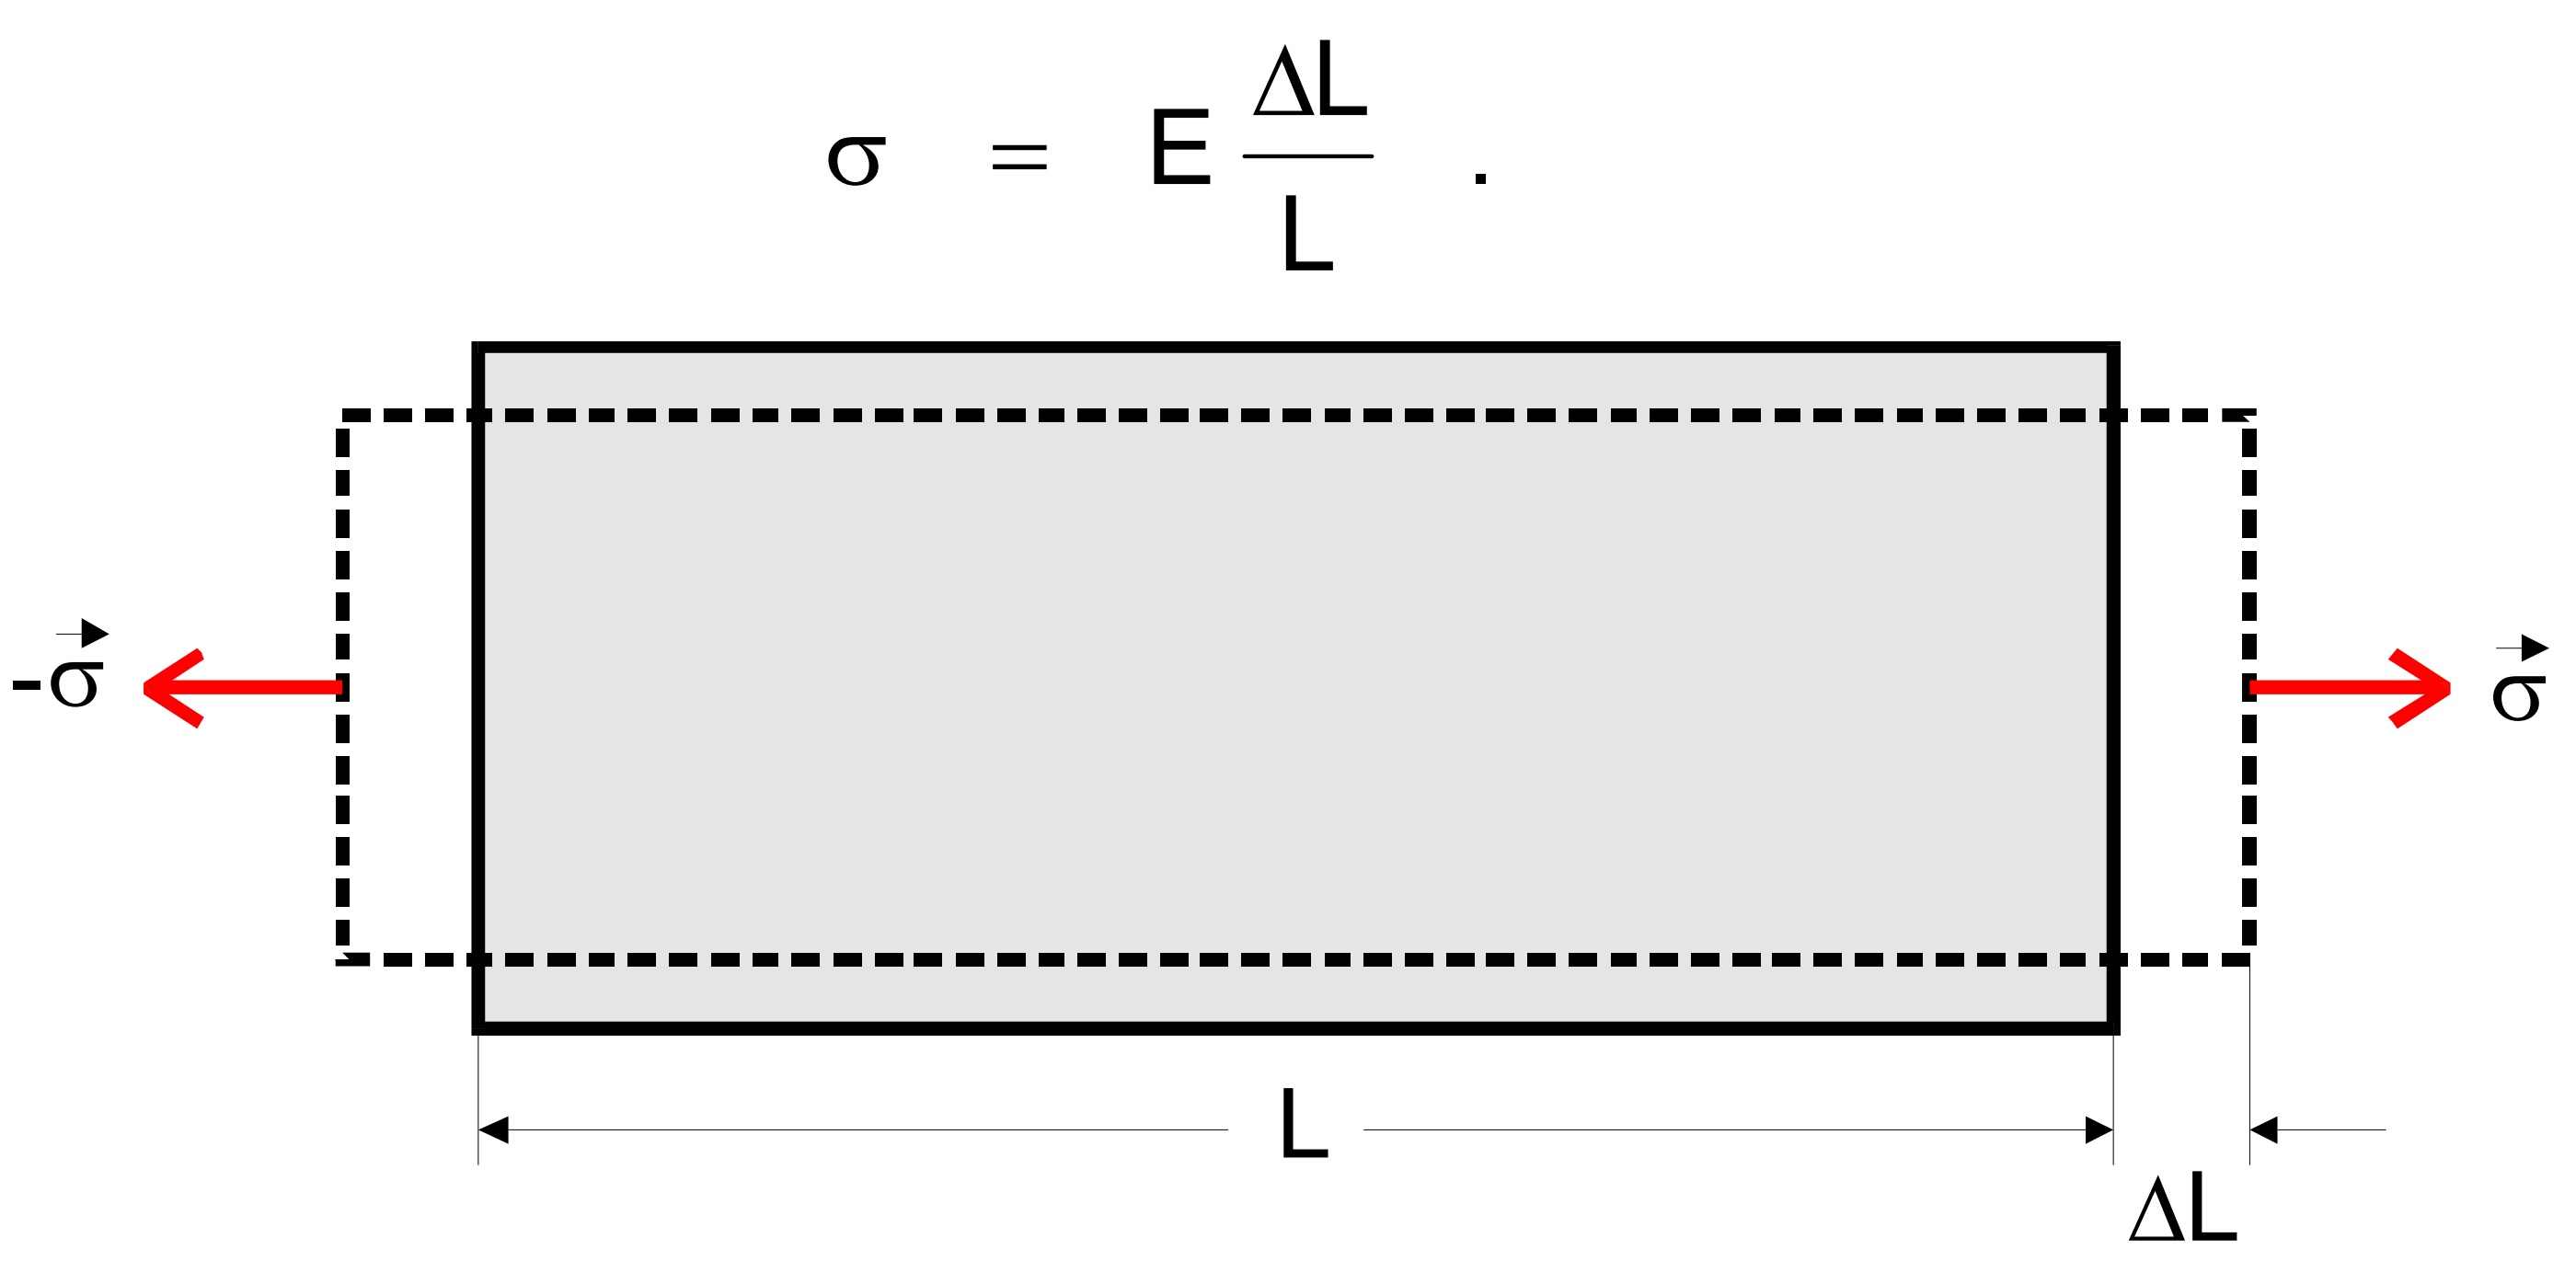
\includegraphics[width=\textwidth]{Bild1.jpg}
\caption{Objekte mit deren Trägheitsmoment}[1]
\label{fig:Abb1}
\end{figure}
Ist die Drehachse nicht durch den Schwerpunkt eines Körpers sondern parallel mit einem Abstand a
zur gehenden Achse verschoben, so lässt sich das Trägheitsmoment mithilfe von Satz des Steiners
\begin{equation}
  I = I_\text{0} + m*a^2
\end{equation}
erechnen. Dabei ist $I_\text{0}$ das Trägheitsmoment der Drehachse durch den Schwerpunkt des Körpers.
Greift eine Kraft mit einem Abstand r von der Achse auf ein drehenden Körper, so wirkt ein Drehmoment $\vec{M} = \vec{F} \times \vec{r}$.
In einem Schwingungssystem wirkt auf ein Körper durch die Drehung um ein Winkel $\phi$ aus seiner Ruhelage ein rücktreibenes Drehmoment
durch eine Feder entgegen. Die harmonische Schwingung lässt sich mit der Schwingungsdauer
\begin{equation}
  T = 2\pi \sqrt{\frac{I}{D}}
\end{equation}
berechnen. I ist dabei das Trägheitsmoment und D die Winkelrichtsgröße.
\begin{equation}
  D = \frac{M}{\phi} \leftrightarrow D = \frac{F \cdot r}{\phi}
\end{equation}
Das harmonische Verhalten bei der Drehschwingung ist nur auf kleinen Winekl $\phi$
beschränkt.

\input{Theorie1.txt}
\input{Theorie2.txt}
\section{Versuchsaufbau}
Zur Bestimmung des Trägheitsmoments I wird zunächst die
die Drillachse, siehe Abbildung 2, benötigt. Die Drillachse
die über eine Spiralfeder mit einem Rahmen verbunden.
\begin{figure}[H]
  \centering
  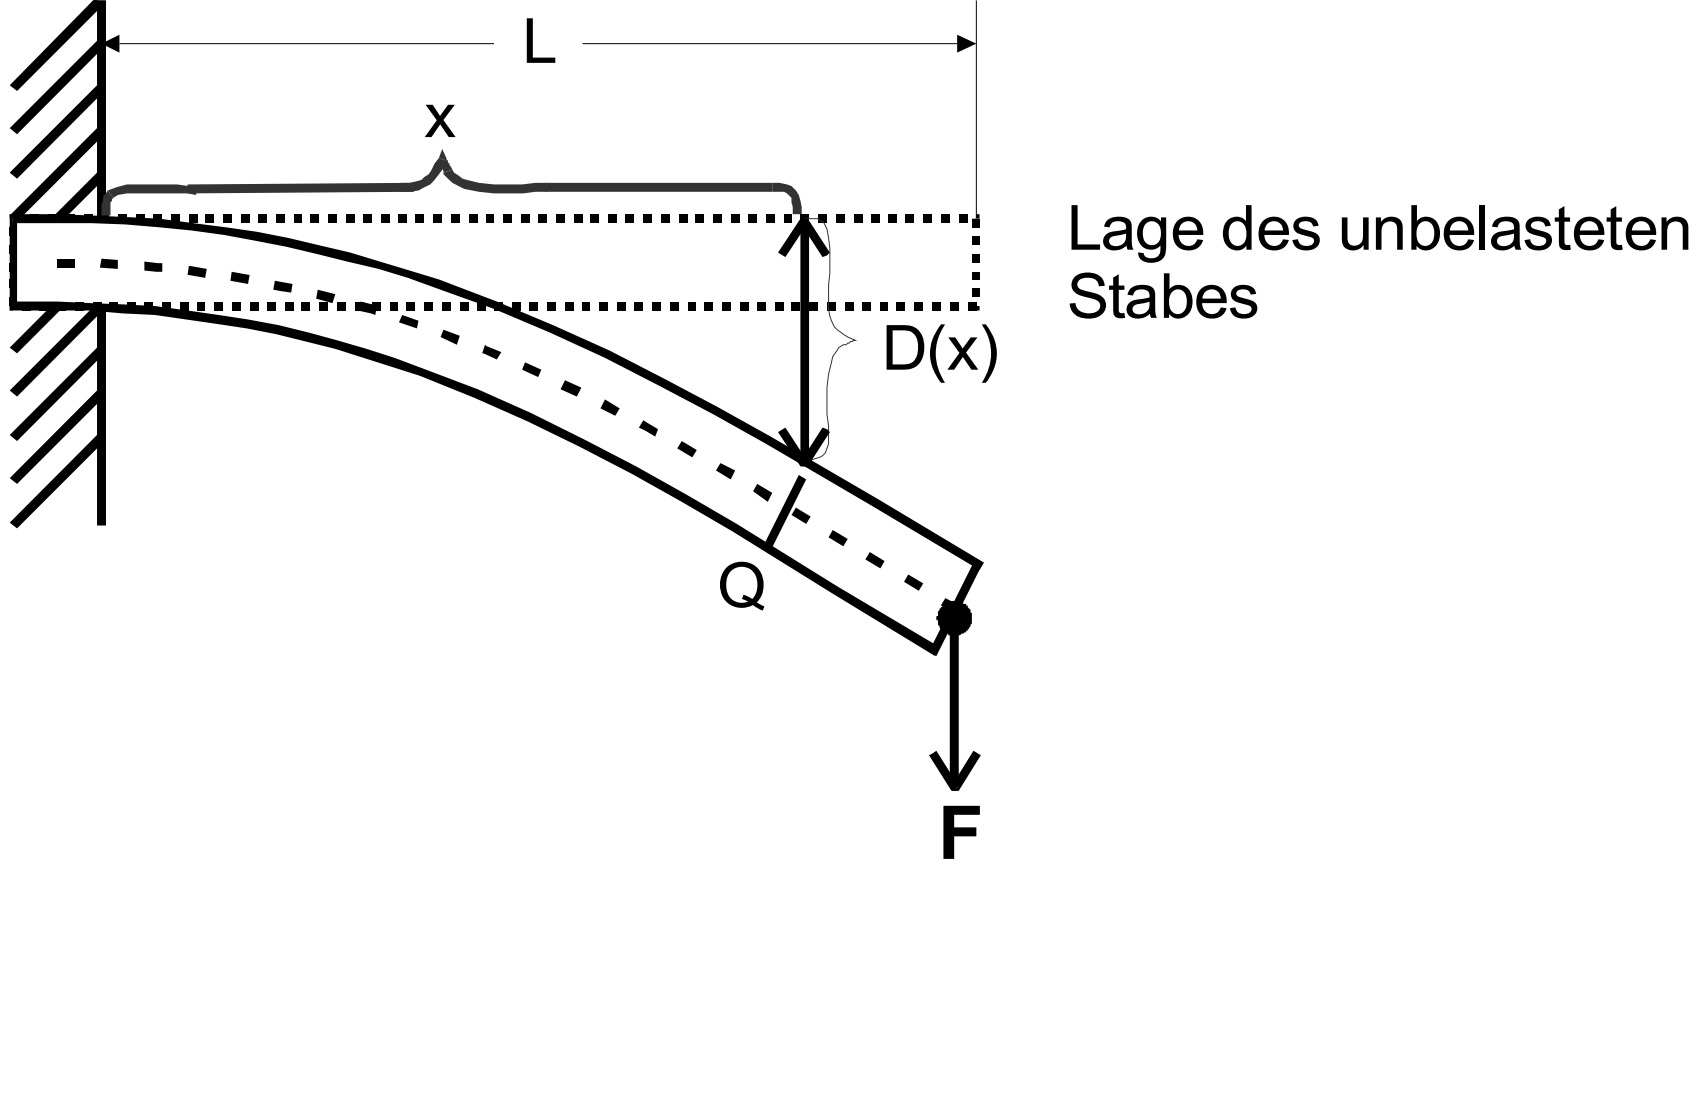
\includegraphics[width=5 cm , height= 10 cm]{Bild2.jpg}
   \caption{Schematische Darstellung des Versuchsaufbau}
\end{figure}
Auf die Achse können verschiedene Objekte angebracht werden.
%Das Eigenträgheitsmoment $I_\text{D}$ sowie die Winkelrichtgröße D lässt sich über die Schwingungsdauer T
%berechnet.

 \section{Durchführung}

\section{Auswertung}
\subsection{Quadratischer Stab bei einseitiger Aufhängung}

Vor der Bestimmung des Elastizitätsmoduls muss zunächst das Material des Stabes bestimmt werden.
Das geschieht über die Dichte des Stabes, welche mit folgender Formel bestimmt werden kann:

\begin{equation}
  \rho = \frac{m}{V} = \frac{m}{L \cdot b^2}
\end{equation}

Die geometrischen Abmessungen des quadratischen Stabes sind:

\begin{enumerate}
  \item Länge: L=\SI{55}{\centi\meter} = \SI{0.55}{\meter}
  \item Masse: m=\SI{435.5e-3}{\kilo\gram}
  \item Breite:
    \begin{enumerate}
      \item Messwerte: \SI{10.4}{\milli\meter}, \SI{10.1}{\milli\meter},
      \SI{10.2}{\milli\meter}, \SI{10.1}{\milli\meter}, \SI{10.1}{\milli\meter},
      \SI{10.1}{\milli\meter}, \SI{10.1}{\milli\meter},
      \SI{10.1}{\milli\meter}, \SI{10.1}{\milli\meter}, \SI{10.1}{\milli\meter}
      \item Mittelwert: b = \SI{10.14(3)e-3}{\meter}
    \end{enumerate}
\end{enumerate}

Der Mittelwert der Breite wird mit dieser Gleichung bestimmt:

\begin{equation}
  \bar{x} = \frac{1}{N} \sum_{i=0}^{N} x_i
\end{equation}

Daraufhin wird die Standartabweichung von dem Mittelwert ermittelt:

\begin{equation}
  \sigma = \frac{1}{\sqrt{N}\sqrt{N-1}} \sqrt{\sum_{i}(x_i-\bar{x})^2}
\end{equation}

Nun ergibt sich für den quadratischen Stab die Dichte:\\
\centerline{$\rho = 7701,04 \pm 45,57 \si[per-mode=fraction]{\kilo\gram\per\metre\tothe{3}}$}

Der Fehler der Dichte lässt sich mithilfe der Gauß´schen Fehlerfortpflanzung berechnen:

\begin{equation}
  \Delta \rho = \sqrt{\left(\frac{\partial\rho}{\partial b} \cdot \Delta b \right)^2}
\end{equation}

Wenn dieser Wert mit Literaturwerten verglichen wird folgt, dass die Dichte von Eisen
am ähnlichsten ist.\\
\centerline{$\rho_{E} = 7860 \si[per-mode=fraction]{\kilo\gram\per\metre\tothe{3}}$ \, [2]}


Mithilfe der Messwerte, die in Tabelle 1 dargestellt sind, lässt sich nun eine
Ausgleichsrechnung durchführen um das Elastizitätsmodul zu bestimmen. Dafür wird die
Durchbiegung D(x) und $\left( Lx^2- \frac{x^3}{3} \right)$ im Plot aufgetragen.
Die Ausgleichsgerade wird mithilfe von Python 3.6 bestimmt.
Die Parameter der Ausgleichsgerade sind:\\

\begin{equation}
  y=mx+b
\end{equation}

\begin{itemize}
  \item m = \SI{33.557(547)e-3}{\meter\tothe{-2}}
  \item b = \SI{5.45(224)e-5}{\meter}
\end{itemize}

Durch Vergleichen von den Gleichungen (1) und (9) folgt für das Elastizitätsmodul:\\

\begin{equation}
  m = \frac{F}{2EI} \iff E= \frac{F}{2mI}
\end{equation}

Das Flächenträgheitsmoment $I$ lässt sich mit der oben genannten Formel bestimmen:\\

\centerline{$I_{quadrat} = \frac{b^4}{12} = \SI{8.81(10)e-10}{\meter\tothe{4}}$}\ \\

Der Fehler wird wieder mit der Gauß´schen Fehlerfortpflanzung bestimmt, wie folgt bestimmt:\\\\

$\Delta I_{quadrat} = \sqrt{\left( \frac{b^3}{3} \cdot \Delta b\right)^2}$\\\\

\begin{table}
  \centering
  \caption{Tabelle mit Messdaten und Daten für die Ausgleichsrechnung.}
  \begin{tabular}{c c c}
    \toprule
    x in \si{\meter} & D(x) in $10^{-3}\si{\meter}$ & $\left(Lx^2-\frac{x^3}{3}\right) \text{in} \, 10^{-3}\si{\meter\tothe{3}}$ \\
    \midrule
    0.03 & 0.03 &  0.486 \\
    0.05 & 0.04 &  1.33 \\
    0.10 & 0.24 &  5.17 \\
    0.15 & 0.47 &  11.25 \\
    0.20 & 0.75 &  19.33 \\
    0.25 & 1.07 &  29.17 \\
    0.30 & 1.4 &  40.5 \\
    0.35 & 1.88 &  53.08 \\
    0.40 & 2.22 &  66.66 \\
    0.45 & 2.78 &  81 \\
    \bottomrule
  \end{tabular}
\end{table}

\begin{figure}[H]
  \centering
  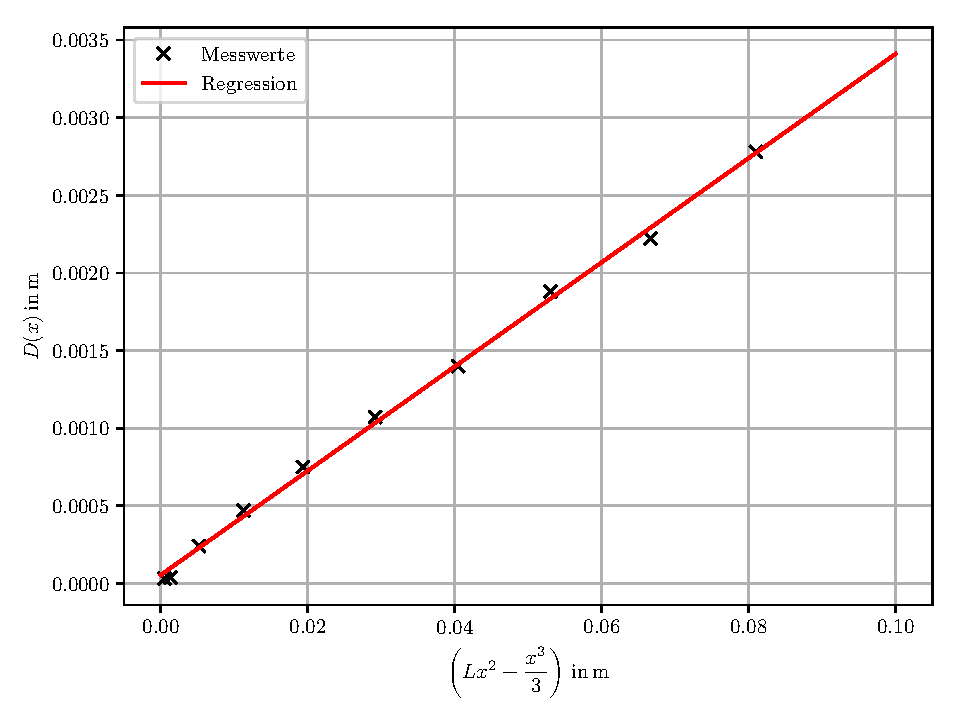
\includegraphics[width=\textwidth]{ausgleichsgerade1.pdf}
  \caption{Messwerte des quadratischen Stabes mit linearer Regression.}
\end{figure}

Die Kraft F ist die Gewichtskraft des verwendeten Gewichtes. In diesen Fall ist das Gewicht
$m_0 = \SI{534.5e-3}{\kilo\gram}$ also ergibt sich für die Gewichtskraft:\\
\centerline{$F = m_0 \cdot g = 5,234 N$}

Nun lässt sich das Elastizitätsmodul des quadratischen Stabes bestimmen und der Fehler
wird wieder mit der Gauß´schen Fehlerfortpflanzung berechnet:

\begin{equation}
  \Delta E = \sqrt{\left(\frac{\partial E}{\partial m} \cdot \Delta m \right)^2 +
  \left( \frac{\partial E}{\partial} I \cdot \Delta I \right)^2}
\end{equation}

Also ist das Elastizitätsmodul: \\
\centerline{$E = \num{88.7(18)e9} \frac{N}{m^2}$}

\subsection{Runder Stab mit einseitiger Aufhängung}

Bei dem Runden Stab muss zunächst wieder die Dichte bestimmt werden um das Material
ungefähr bestimmen zu können. Die geometrischen Abmessungen des runden Stabes sind:

\begin{enumerate}
  \item Länge L = \SI{0.55}{\meter}
  \item Masse m = \SI{121.3e-3}{\kilo\gram}
  \item Durchmesser:
  \begin{enumerate}
    \item Messwerte: \SI{10}{\milli\meter}, \SI{10}{\milli\meter}, \SI{10}{\milli\meter},
    \SI{10}{\milli\meter}, \SI{10}{\milli\meter}, \SI{10}{\milli\meter},
    \SI{10}{\milli\meter}, \SI{10}{\milli\meter}, \SI{10}{\milli\meter},
    \SI{10}{\milli\meter}, \SI{10}{\milli\meter}
    \item Mittelwert: d = \SI{10e-3}{\meter}
  \end{enumerate}
\end{enumerate}

Der Mittelwert wird mithilfe der Gleichung (6) berechnet aber da alle Messwerte gleich
sind ist der Mittelwert das gleiche wie die Messwerte und hat keinen Fehler.

Die Dichte des runden Stabes lässt sich nun mit der folgenden Gleichung bestimmen:

\begin{equation}
  \rho = \frac{m}{V} = \frac{m}{L \pi \frac{d^2}{4}}
\end{equation}

Somit ergibt sich für die Dichte:\\
\centerline{$\rho = \SI[per-mode=fraction]{2808.07}{\kilo\gram\per\meter
\tothe{3}}$}

Diese Dichte wird wieder mit Literaturwerten verglichen und es folgt, dass die Dichte
von Aluminium am ähnlichsten ist:\\
\centerline{$\rho_A = \SI[per-mode=fraction]{2710}{\kilo\gram\per\meter
\tothe{3}}$ \, [2]}

\begin{table}
  \centering
  \caption{Tabelle mit Messdaten und Daten für die Ausgleichsrechnung.}
  \begin{tabular}{c c c}
  \toprule
  $x$ in \si{\meter} & $D(x) \text{in} \, 10^{-3}\si{\meter}$ & $\left(Lx^2-\frac{x^3}{3}\right) \text{in} \, 10^{-3}\si{\meter\tothe{3}}$ \\
  \midrule
  0.03 & 0.05 &   0.486 \\
  0.05 & 0.1 & 1.33 \\
  0.10 & 0.42 &   5.17 \\
  0.15 & 0.82 &   11.25 \\
  0.20 & 2.1  & 19.33 \\
  0.25 & 1.99 &   29.17 \\
  0.30 & 2.62 &   40.5 \\
  0.35 & 3.42 &   53.08 \\
  0.40 & 4.13 &   66.66 \\
  0.45 & 4.93 &   81 \\
  \bottomrule
  \end{tabular}
\end{table}

In der Tabelle 2 sind die Messwerte für den runden Stab dargestellt. Nun wird wieder
die Durchbiegung D(x) und die Werte zum Term $\left(Lx^2-\frac{x^3}{3}\right)$ in
einem Plot dargestellt und es wird eine Ausgleichsrechnung durchgeführt.

\begin{figure}[H]
  \centering
  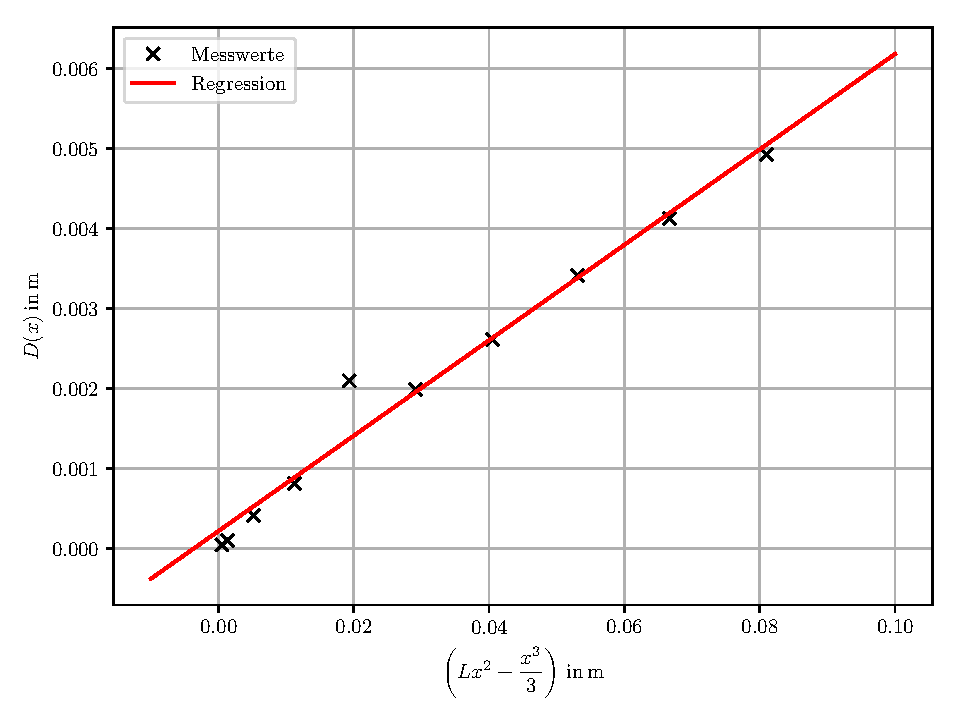
\includegraphics[width=\textwidth]{ausgleichsgerade2.pdf}
  \caption{Messwerte des runden Stabes mit linearer Regression.}
\end{figure}

Die Parameter der Ausgleichsgeraden werden wieder mithilfe von Python 3.6 ermittelt:

\begin{itemize}
  \item m = \SI{59.623(3313)e-3}{\meter\tothe{-2}}
  \item b = \SI{22.17(1559)e-5}{\meter}
\end{itemize}

Durch Vergleichen der Gleichungen (5) und (18) ergibt sich wieder die Gleichung (19).

Die Formel für das Flächenträgheitsmoment eines runden Stabes lässt sich auch mit
der oben genannten Gleichung ermitteln:\\

\centerline{$I_{Rund} = \frac{\pi}{4} R^4 = \SI{490.87e-12}{\meter\tothe{4}}$}\ \\

Die Gewichtskraft für den runden Stab ist die gleiche wie bei dem quadratischen,
da die Masse des Gewichtes gleich ist. F ist also $5,243N$.

Das Elastizitätsmodul des runden Stabes lässt sich nun bestimmen und der Fehler
wird mit der Gleichung (19) berechnet.\\

\centerline{$E = \num{90(5)e9} \frac{N}{m^2}$}

\subsection{Quadratischer Stab mit beidseitiger Aufhängung}

Bei der Bestimmung des Elastizitätsmoduls durch beidseitige Aufhängung müssen zwei
Fälle betrachtet werden. Zunächst wird die Durchbiegung von $0$ bis $\frac{L}{2}$
durch die Gleichung (12) beschrieben. Der Teil von $\frac{L}{2}$ bis $L$ wird seperat
durch die Gleichung (13) beschrieben.

Für beide Hälften des Stabes lässt sich nun eine Ausgleichsrechnung durchführen
und jeweils ein Elastizitätsmodul bestimmen. Im idealfall sollten die
Elastizitätsmodule gleich sein.

Zunächst wird das Elastizitätsmodul für $0$ bis $\frac{L}{2}$ bestimmt.

\begin{table}
  \centering
  \caption{Tabelle mit Messdaten und Daten von $0$ bis $\frac{L}{2}$.}
  \begin{tabular}{c c c}
    \toprule
    x in \si{\meter} & $D(x) \text{in} \, 10^{-3} \si{\meter}$ &
    $ \left( 3L^2x-4x^3 \right) \text{in} \, 10^{-3} \si{\meter\tothe{3}}$\\
    \midrule
    0    & -0.03 & 0 \\
    0.05 & 0.24 & 44.87 \\
    0.10 & 0.42 & 86.75 \\
    0.15 & 0.66 & 122.625 \\
    0.20 & 0.89 & 149.5 \\
    0.25 & 0.88 & 164.375 \\
    \bottomrule
  \end{tabular}
\end{table}

\begin{figure}[H]
  \centering
  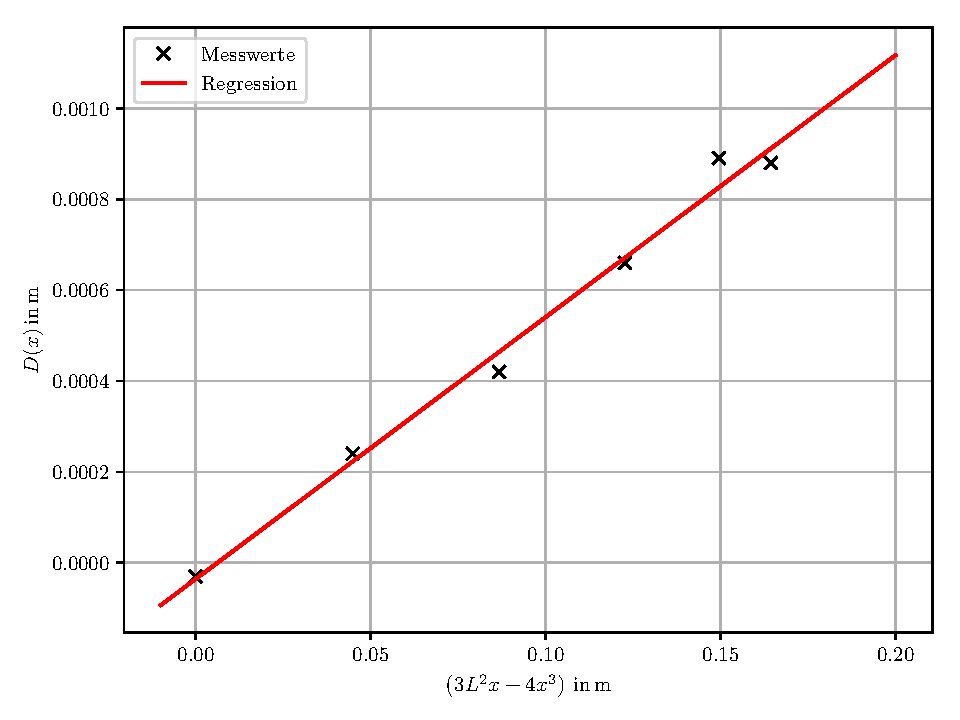
\includegraphics[width=\textwidth]{ausgleichsgerade3.pdf}
  \caption{Messwerte des quadratischen Stabes für $0$ bis $\frac{L}{2}$ mit linearer Regression.}
\end{figure}

Die Ergebnisse der Ausgleichsrechnung, die wieder mit Python 3.6 durchgeführt wurde,
lauten:

\begin{itemize}
  \item $m = \SI{5.761(305)e-3}{\meter\tothe{-2}}$
  \item $b = \SI{-3.6(34)e-5}{\meter}$
\end{itemize}

Für die Berechnung des Elastizitätsmoduls werden die Gleichungen (18) und (12)
verglichen. Dadurch ergibt sich wieder die Gleichung (19) für das Elastizitätsmodul.
Das Flächenträgheitsmoment für den quadratischen Stab wurde bereits berechnet.

Die Gewichtskraft ist diesmal jedoch anders, da die Masse $m_1 = \SI{2.362}{\kilo\gram}$
beträgt. Daraus ergibt sich dann die Kraft $F = 23,171N$.

Nun lässt sich das Elastizitätsmodul für den ersten Teil der Messung bestimmen,
die mit der folgenden Gleichung berechnet wird:

\begin{equation}
  m = \frac{F}{48EI} \iff E = \frac{F}{48mI}
\end{equation}

\centerline{$E = \num{95(5)e9} \frac{N}{m^2}$}\ \\

Der Fehler wird mit der Gauß´schen Fehlerfortpflanzung bestimmt:\\\\

$\Delta E = \sqrt{\left(\frac{-F}{48m^2I}\cdot \Delta m \right)^2 + \left(
\frac{-F}{48mI^2} \cdot \Delta I \right)^2}$\\\\

Für den zweiten Teil der Messung von $\frac{L}{2}$ bis $L$ sind die Rechnungen
identisch nur, dass die Gleichung (13) anstatt (12) verwendet wird.

\begin{table}
  \centering
  \caption{Tabelle mit Messdaten und Daten von $\frac{L}{2}$ bis $L$.}
  \begin{tabular}{c c c}
    \toprule
    x in \si{\meter} & $D(x) \text{in} \, 10^{-3} \si{\meter}$ &
    $ \left( 4x^3-12Lx^2+9L^2x-L^3 \right) \text{in} \, 10^{-3} \si{\meter\tothe{3}}$\\
    \midrule
    0.30 & 1.73 & 164.375 \\
    0.35 & 1.67 & 149.5 \\
    0.40 & 1.57 & 122.625 \\
    0.45 & 1.37 & 86.75 \\
    0.50 & 1.15 & 44.875 \\
    \bottomrule
  \end{tabular}
\end{table}

\begin{figure}[H]
  \centering
  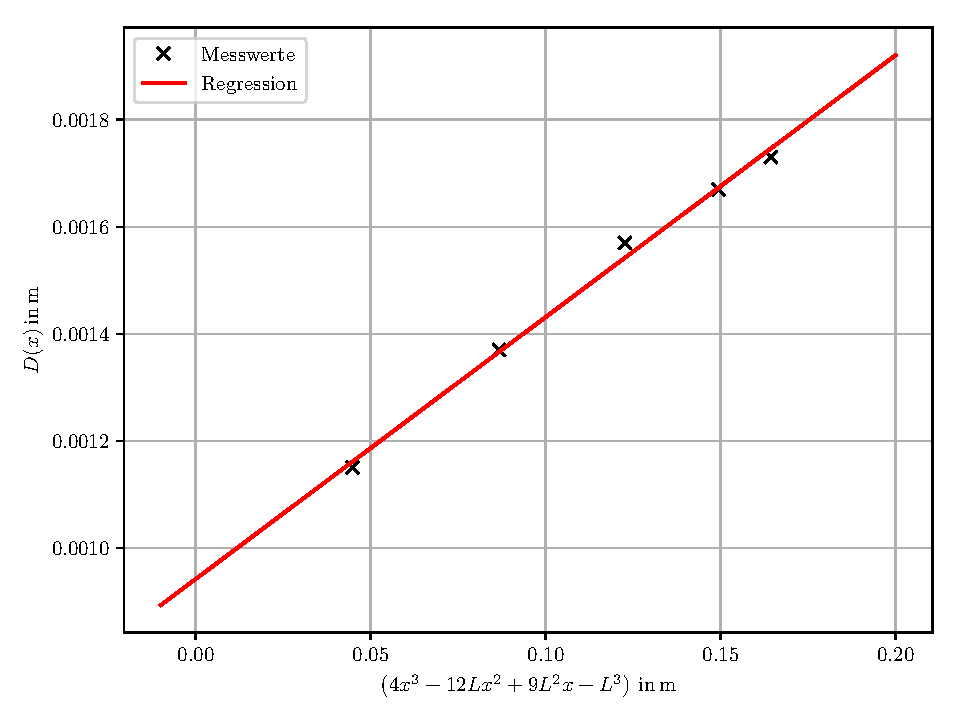
\includegraphics[width=\textwidth]{ausgleichsgerade3.1.pdf}
  \caption{Messwerte des quadratischen Stabes für $\frac{L}{2}$ bis $L$ mit linearer Regression.}
\end{figure}

Damit lauten die Parameter der Ausgleichsgeraden, die mit Python 3.6 bestimmt wurden:

\begin{itemize}
  \item $m = \SI{4.893(207)e-3}{\meter\tothe{-2}}$
  \item $b = \SI{94.2(25)e-5}{\meter}$
\end{itemize}


Da alle Rechnungen gleich sind lässt sich sofort das Elastizitätsmodul für den
zweiten Teil der Messungen angeben:\\

\centerline{$E = \num{112(5)e9} \frac{N}{m^2}$}


\subsection{Runder Stab mit beidseitiger Aufhängung}

Für die Bestimmung des Elastizitätsmoduls für den runden Stab bei beidseitiger
Aufhängung müssen wieder zwei Ausgleichsrechnungen durchgeführt werden, für
$0$ bis $\frac{L}{2}$ und für $\frac{L}{2}$ bis $L$. Die verwendeten Formeln sind
die gleichen wie bei dem quadratischen Stab.

Zunächst wird für den ersten Fall $0$ bis $\frac{L}{2}$ die Ausgleichsrechnung
durchgeführt.

\begin{table}
  \centering
  \caption{Tabelle mit Messdaten und Daten von $0$ bis $\frac{L}{2}$.}
  \begin{tabular}{c c c}
    \toprule
    x in \si{\meter} & $D(x) \text{in} \, 10^{-3} \si{\meter}$ &
    $ \left( 3L^2x-4x^3 \right) \text{in} \, 10^{-3} \si{\meter\tothe{3}}$\\
    \midrule
    0    & 0    &  0 \\
    0.05 & 0.6 & 44.87 \\
    0.10 & 1.02 &  86.75 \\
    0.15 & 1.47 &  122.625 \\
    0.20 & 1.76 &  149.5 \\
    0.25 & 1.92 &  164.375 \\
    \bottomrule
  \end{tabular}
\end{table}

\begin{figure}[H]
  \centering
  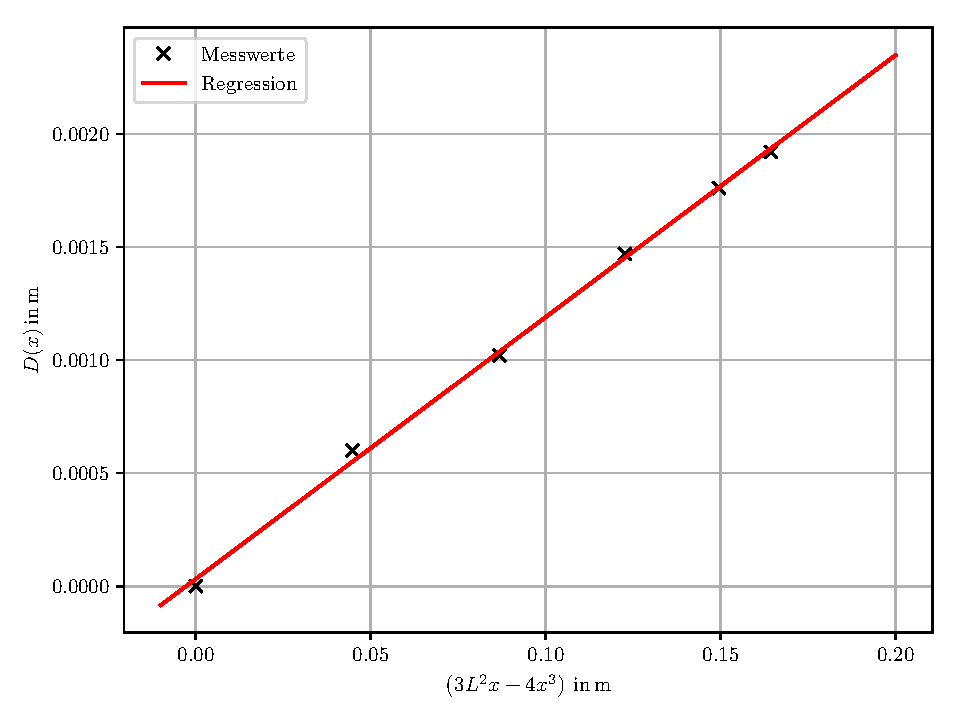
\includegraphics[width=\textwidth]{ausgleichsgerade4.pdf}
  \caption{Messwerte des runden Stabes für $0$ bis $\frac{L}{2}$ mit linearer Regression.}
\end{figure}

Nun wird die Ausgleichsrechnung mithilfe von Python 3.6 durchgeführt, womit die Parameter
der Ausgleichsgeraden bestimmt wird:

\begin{itemize}
  \item $m = \SI{11.580(229)e-3}{\meter\tothe{-2}}$
  \item $b = \SI{3.2(25)e-5}{\meter}$
\end{itemize}

Die Rechnungen und Formeln zur bestimmung des Elastizitätsmoduls sind identisch mit
denen die für den quadratischen Stab benutzt wurden. Deshalb lässt sich das Elastizitätsmodul
direkt angeben:

\centerline{$E= \num{84.9(22)e9} \frac{N}{m^2}$}

Das Vorgehen für die Bestimmung des Elastizitätsmoduls für den zweiten Teil der
Messungen ist wieder gleich mit dem für den quadratischen Stab.

\begin{table}
  \centering
  \caption{Tabelle mit Messdaten und Daten von $\frac{L}{2}$ bis $L$.}
  \begin{tabular}{c c c}
    \toprule
    x in \si{\meter} & $D(x) \text{in} \, 10^{-3} \si{\meter}$ &
    $ \left( 4x^3-12Lx^2+9L^2x-L^3 \right) \text{in} \, 10^{-3} \si{\meter\tothe{3}}$\\
    \midrule
    0.30 & 2.77 &  164.375 \\
    0.35 & 2.64 &  149.5 \\
    0.40 & 2.36 &  122.625 \\
    0.45 & 1.91 &  86.75 \\
    0.50 & 1.4 & 44.875 \\
    \bottomrule
  \end{tabular}
\end{table}

\begin{figure}[H]
  \centering
  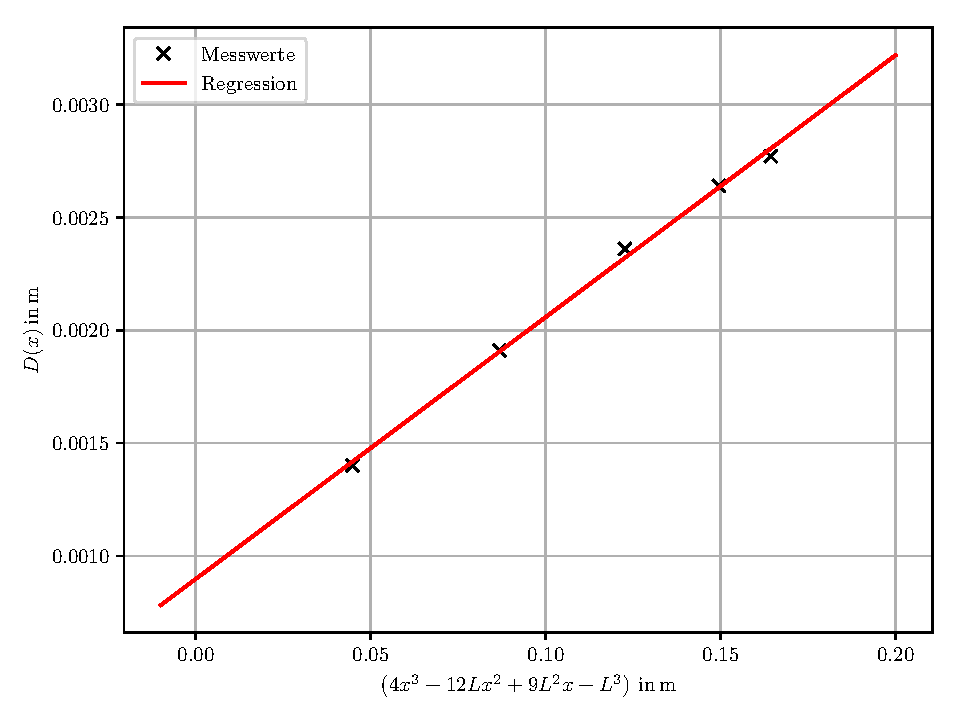
\includegraphics[width=\textwidth]{ausgleichsgerade4.1.pdf}
  \caption{Messwerte des runden Stabes für $\frac{L}{2}$ bis $L$ mit linearer Regression.}
\end{figure}

Mithilfe der Messwerte, die in Tabelle 1 dargestellt sind, lässt sich nun eine
Ausgleichsrechnung durchführen um das Elastizitätsmodul zu bestimmen. Die Ausgleichsgerade
wird mithilfe von Python 3.6 bestimmt.

\begin{itemize}
  \item $m = \SI{11.599(337)e-3}{\meter\tothe{-2}}$
  \item $b = \SI{89.8(41)e-5}{\meter}$
\end{itemize}


Damit lässt sich nun das Elastizitätsmodul des runden Stabes noch einmal bestimmen,
mithilfe der Überlegungen für den quadratischen Stab:

\centerline{$E= \num{84.8(25)e9} \frac{N}{m^2}$}

\section{Diskussion}

In der Auswertung wurden die Dichten der zwei Stäbe bestimmt und somit das Material
näherungsweise bestimmt.

Für den quadratischen Stab wurde Eistenstahl als Material angenommen. Der Literaturwert
des Elastizitätsmoduls von Eisenstahl beträgt $E = \num{196e9} \frac{N}{m^2}$. Damit weicht der
gemessene Wert um $\SI{42.9}{\percent} - \SI{54.7}{\percent} $ von dem Literaturwert ab.

Bei dem Runden Stab wurde Aluminium als Material bestimmt. Der Literaturwert ist in diesem
Fall $E = \num{70e9} \frac{N}{m^2}$. Die Abweichung der gemessenen Werte liegt also zwischen
\SI{21.1}{\percent} und \SI{28.6}{\percent}.

Es wird direkt klar, dass es eine Abweichung zu den Literaturwerten geben muss, da
die einzelnen Elastizitätsmodule, die mit unterschiedlichen Methoden bestimmt worden
sind zum Teil sehr unterschiedlich sind.
Diese Fehler könnten durch die Fehlerhafte Messung der Durchbiegung entstanden sein.
Die verwendeten Messuhren waren zum Teil etwas ungenau und die Werte waren auch
schwierig abzulesen.
Außerdem könnte die Bestimmung des Materials auch falsch gewesen sein, da bei dem
quadratischen Stab die gemessene Dichte stark von einer Dichte eines möglichen Materials
abweicht.

\end{document}
